\section{Seven Parameter Solar Cell Model}\label{sec:seven_parameter_solar_cell_model}


\begin{figure}[h]
    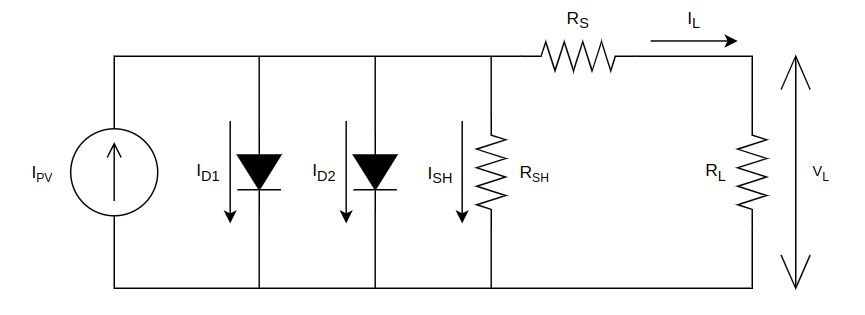
\includegraphics[width=\textwidth]{solar_cell_seven_parameter_model.png}
    \caption{Seven Parameter, or Double Diode Model of a Solar Cell}
    \label{fig:double_diode_model}
\end{figure}

The seven parameter solar cell model, also known as a double diode model, shown
in Figure~\ref{fig:double_diode_model}, builds upon the five parameter model by
introducing a second diode (hence the name) to more accurately model internal
current losses, which can be split into the following:

\begin{itemize}
    \item losses due to carrier recombination in the space charge region of the
    P-N junction,
    \item and losses due to surface recombination.
\end{itemize}

These currents are denoted the \ac{ID1} and \ac{ID2}, respectively. By
differentiating between the two primary recombination processes in the cell, the
seven parameter model is generally considered more accurate than the five
parameter model.
